\documentclass[Softwaredesign/Softwaredesign_main.tex]{subfiles}
\begin{document}
\subsection{Design af CupLight\_IF} \label{sec:cuplight_sw_design}
Til at kontrollere lyset under kopperne, skal der bruges et interface, der kan anvendes fra PlayerSideController-klassen. Dette kapitel vil præsentere nogle af de design valg, der er lavet vedrørende det interface, samt en sammenligning mellem de forskellige teknologier, der præsenteres. De forskellige designs er lavet ud fra Hardware Designs, der kan ses i \fullref{hwdesign:sec:cuplight_hw_design}.
\subsubsection{CupLight\_IF Software Design ved multiplexing}
Da pointen ved at bruge en RGB-led er, at der kan styres farven af led'en så skal der laves  et modul \textit{rgb\_led}, som har til formål at stå for at håndtere farverne i en RGB-led. Som sagt kan farven på en RGB-led styres ved at bruge PWM på benene, så derfor skal den kunne styre 3 pwm generatorer i PSoC creator. Tilhørende til dette modul laves en typedef struktur kaldet \textit{color\_t}, der er en definition af hvad farverne indeholder. Farverne der er i den valgte RGB-led er som navnet hentyder, rød,grøn og blå. Farverne hertil kan kun have værdier mellem 0 og 255, hvilket der bør tages hånd om når en farve tildeles en værdi.
\\ PWM-generatorne kan i sig selv styre en enkelt LED, og bør derfor passende testes for dette. I princippet kan den også styre flere LED'er, men dette er ikke relevant i dette system, da alle LED'er vil have samme farve.
\\Til at kontrollere flere LED'er til forskellige farver bruges PSoC's SPI Master komponent, da denne kan bruges til at kommunikere med det hardware komponent, der er givet fra hardware designet \fullref{hwdesign:sec:cuplight_hw_design}. Derudover skal der være en digital output pin, der har til formål at latche outputtet, samt en pin, der har til formål at enable outputtet på registeret. Det samlede design for komponenterne, der er anvendt i PsoC'en kan ses på figur \ref{fig:CupLight_PSoC_Design}.
\begin{figure}[H]
    \centering
    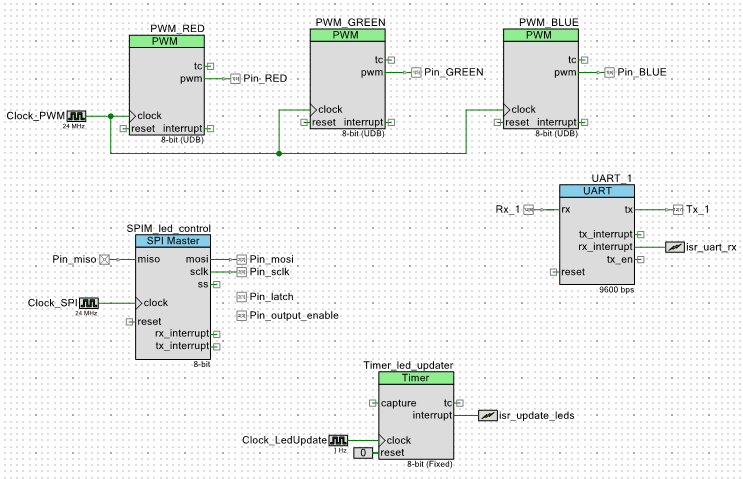
\includegraphics[width=\textwidth]{Softwaredesign/CupLight_IF/graphics/CupLightPSoCDesign.png}
    \caption{PSoC design for CupLight\_IF}
    \label{fig:CupLight_PSoC_Design}
\end{figure}

Der anvendes et SPI Master komponent, men ikke en egentlig protokol for SPI, da SPI-slaven bare bruges til at tænde for en af sine pins en efter en, for at opnå multiplexing.

\subsubsection{ShiftPWM}
Til denne implementering kræves, der noget avanceret bit shifting, i det der skal laves et PWM signal på de forskellige pins. Hertil laves et modul, der hedder ShiftPWM, som har til ansvar at stå for at lave ShiftRegisteret til en PWM generator. Her skal der igen anvendes et SPI Master komponent på PSoC'en for at shifte bits ind i 74HC595, men derudover skal der kun anvendes en timer, der har til formål at interrupte, hver gang der skal ske en opdatering af LED'erne. Det overordnede design kan ses på figur \ref{fig:CupLight_ShiftPWM_PSoC_Design}.

\begin{figure}
    \centering
    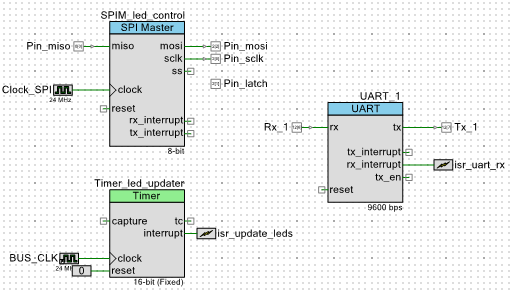
\includegraphics{Softwaredesign/CupLight_IF/graphics/CupLightPSoCDesign_ShiftPWM.png}
    \caption{PSoC desing for CupLight\_IF, der anvender ShiftPWM}
    \label{fig:CupLight_ShiftPWM_PSoC_Design}
\end{figure}

Det ses af figur \ref{fig:CupLight_ShiftPWM_PSoC_Design}, at en fordel ved dette desing er, at der er færre komponenter anvendt på PSoC'en (Kun 2, hvis UART til debugging ikke tælles med). Den klare ulempe ved dette design er kompleksiteten af måden, hvorpå der sendes de rigtige værdier over SPI.\\
Til at sende de rigtige bits kan anvendes en global datastruktur, men den har en ulempe omkring memory, idet den fylder $ShiftRegData[Resolution \cdot nShiftRegisters]$, hvor resolution er de ønskede steps på PWM signalet og nShiftregisters er antallet 74HC595, der er daisy chained. Det største problem ved denne løsning er timeslices. For at lave et PWM-signal på denne måde, bliver algoritmen, der opdatere shift registeret ud fra datastrukturen nødt til, at være yderst effektiv, i det den kommer til at blive kaldt ofte. Hvis det interrupt, der så kaldes varer for lang tid, så går det ud over hele PlayerSide modulet, da de andre dele ikke har et stort nok timeslice, til at få deres arbejde gjort. Det bedste ved denne løsning er muligheden for at udvide lyset i systemet. Udover den øvre grænse for antallet af Daisy Chained shift registeret og den lille forlængelse af time-slice, så påvirker det ikke styrken af lyset, at der er flere LED'er, som det ville ved Multiplexing.Der skal også lægges mærke til at timeslice for interruptet må stige lineært i forhold til antallet af skifteregistre. Der er derfor også en mulighed for at styre de individuelle LED'er i hver CupHolder, hvis det var ønsket.

\subsubsection{Diskussion af Multiplexing vs. ShiftPMW}
I dete afsnit diskuteres hvorvidt multiplexing eller ShiftPWM anvendes for det pågældende projekt.\\
Starter vi ud med at kigge på \textbf{Multiplexing} så er der nogle klare fordele, så som mindre memory brug og det er nemmere at implementere. Derudover vil den ikke bruge lige så store timeslices, som ved ShiftPwm. Men det har også nogle ulemper, så som at der er meget af fintuning af timing for lyset og at lyset bliver mindre kraftigt. Fintuningen af timingen kan komme til at have alvorlige konsekvenser for lyset, da det er meget følsom overfor, de andre moduler på PSoC playerside.
\\Ved \textbf{ShiftPWM} udnyttes der derimod pins på PSoC'en vanvittigt effektiv idet, der kan styre et nærmest vilkårligt antal LED'er (Der er en øvre grænse for, hvor mange shiftregisters der kan daisy chaines og fungere). Derudover vil lysene også være kraftigere og med flere farver, hvor tradeoff er det memory, der skal anvendes til at holde styr på sekvensen af pins, der skal opdateres.
\\Den endelig konklusion er, at det ShiftPWM anvendes, da det bare har for mange fordele i forhold til ulemper i sammenligning med Multiplexing. Da koden er simplere og mere intuitiv, og det samme er hardwaren. Det andet der taler for ShiftPWM er antallet af mulige farver, hvilket opfylder kravene i bilag \fullref{kravspec:sec:ikke_funktionelle_krav} omkring antallet af farver.\\
Nu hvor der er taget et valg omkring teknologi, så kan der laves et klasse diagram for modulet. Denne ses i figur \ref{fig:cd_cuplight}.
\begin{figure}[H]
    \centering
    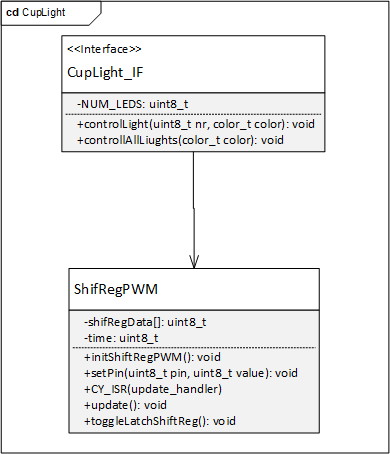
\includegraphics[width=\textwidth]{Softwaredesign/CupLight_IF/graphics/CD_CupLight.png}
    \caption{Klassediagram for CupLight modulet}
    \label{fig:cd_cuplight}
\end{figure}
Ud fra dette klasse diagram, kan der startes en implementering af modulet.



\end{document}